\documentclass[a4]{beamer}
\usepackage{amssymb}
\usepackage{graphicx}
\usepackage{subfigure}
\usepackage{framed}
\usepackage{newlfont}
\usepackage{amsmath,amsthm,amsfonts}
%\usepackage{beamerthemesplit}
\usepackage{pgf,pgfarrows,pgfnodes,pgfautomata,pgfheaps,pgfshade}
\usepackage{mathptmx}  % Font Family
\usepackage{helvet}   % Font Family
\usepackage{color}

\mode<presentation> {
 \usetheme{Frankfurt} % was
 \useinnertheme{rounded}
 \useoutertheme{infolines}
 \usefonttheme{serif}
 %\usecolortheme{wolverine}
% \usecolortheme{rose}
\usefonttheme{structurebold}
}

\setbeamercovered{dynamic}

\title[MA4603]{Science Maths 3 \\ {\normalsize MA4603 Lecture 11A}}
\author[Kevin O'Brien]{Kevin O'Brien \\ {\scriptsize Kevin.obrien@ul.ie}}
\date{Autumn Semester 2017}
\institute[Maths \& Stats]{Dept. of Mathematics \& Statistics, \\ University \textit{of} Limerick}

\renewcommand{\arraystretch}{1.5}

\begin{document}





\begin{frame}
\frametitle{Shapiro-Wilk Test(a)}


\begin{itemize}
\item We will often be required to determine whether or not a data set is normally distributed.
\item This assumption underpins many statistical models.
\item The null hypothesis is that the data set is normally distributed.
\item The alternative hypothesis is that the data set is not normally distributed.
\item One procedure for testing these hypotheses is the Shapiro-Wilk test, implemented in \texttt{R} using the command \texttt{shapiro.test()}.
\item (Remark: You will not be required to compute the test statistic for this test.)
\end{itemize}
\end{frame}
%----------------------------------------%
\begin{frame}[fragile]
	\frametitle{Shapiro-Wilk Test(b)}

\textbf{IMPORTANT}
\begin{itemize}
	\item $H_0$ : The sample is drawn from a population that is normally distributed. 
	\item $H_1$ : The sample is drawn from a population that is NOT normally distributed. 
\end{itemize}
	
\end{frame}
%----------------------------------------%
\begin{frame}[fragile]
\frametitle{Shapiro-Wilk Test(c)}
For the data set used previously; $x$ and $y$, we use the Shapiro-Wilk test to determine that both data sets are normally distributed.
\begin{verbatim}

> shapiro.test(X)

        Shapiro-Wilk normality test

data:  x
W = 0.9474, p-value = 0.6378

> shapiro.test(y)

        Shapiro-Wilk normality test

data:  y
W = 0.9347, p-value = 0.5273
\end{verbatim}
\end{frame}
%----------------------------------------%
\begin{frame}[fragile]
	\frametitle{Shapiro-Wilk Test(c)}
	
\begin{itemize}
	\item If we fail to reject $H_0$ we are saying that there is not enough evidence to contradict the null hypothesis. \smallskip
	\item This is not the same as saying that the data is a sample drawn from a normally distributioned population. \smallskip
	\item This is a common misconception.
	\item Hypothesis Testing is about strength of evidence, not proof.
\end{itemize}
	
	
\end{frame}


%-------------------------------------------------%
\begin{frame}[fragile]
\frametitle{Graphical Procedures for Assessing Normality}

\begin{itemize}
\item The normal probability (Q-Q) plot is a very useful tool for determining whether or not a data set is normally distributed.
\item \textbf{Important} Interpretation is simple. If the points follow the trendline, we can assume that that data set is a sample drawn from a normally distributed population.
%(provided by the second line of \texttt{R} code \texttt{qqline}).
\item One should expect minor deviations. Numerous major deviations would lead the analyst to conclude that the data set is not normally distributed.
\item The Q-Q plot is best used in conjunction with a formal procedure such as the Shapiro-Wilk test.
\end{itemize}

\begin{framed}
\begin{verbatim}
>qqnorm(mySample)
>qqline(mySample)
\end{verbatim}
\end{framed}
\end{frame}

%-------------------------------------------------%

\begin{frame}
\frametitle{Graphical Procedures for Assessing Normality}

\begin{center}
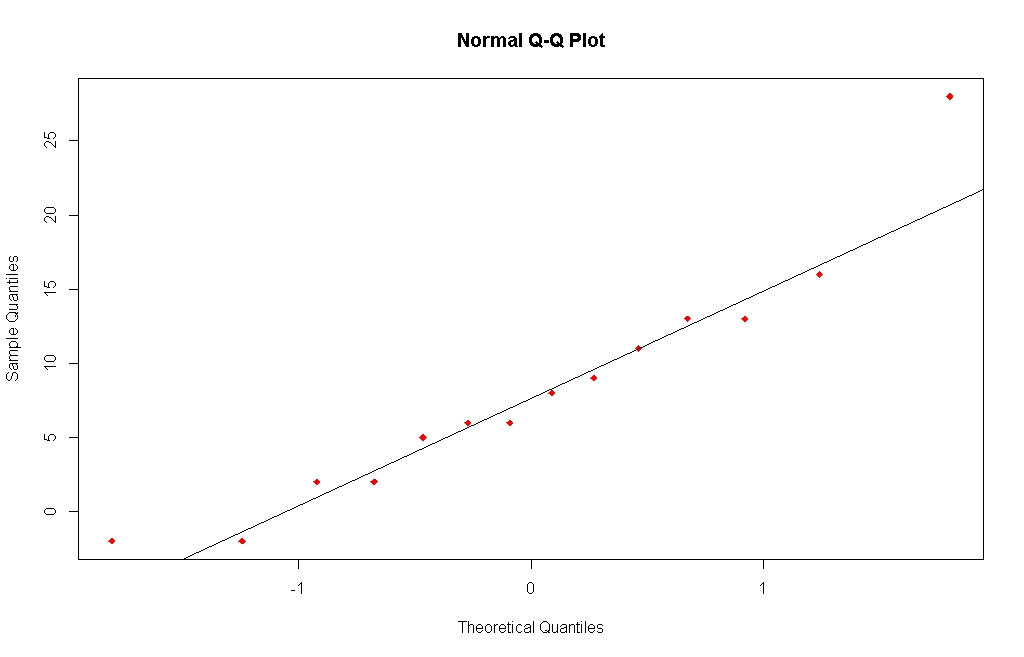
\includegraphics[scale=0.32]{10AQQplot}
\end{center}
\end{frame}


\begin{frame}
	\frametitle{Interpretation: Can NOT Assume Normal Distribution}
	
	\begin{center}
		\includegraphics[scale=0.6]{QQplot2}
	\end{center}
\end{frame}


\begin{frame}
	\frametitle{Graphical Procedures for Assessing Normality}
	
	\begin{center}
		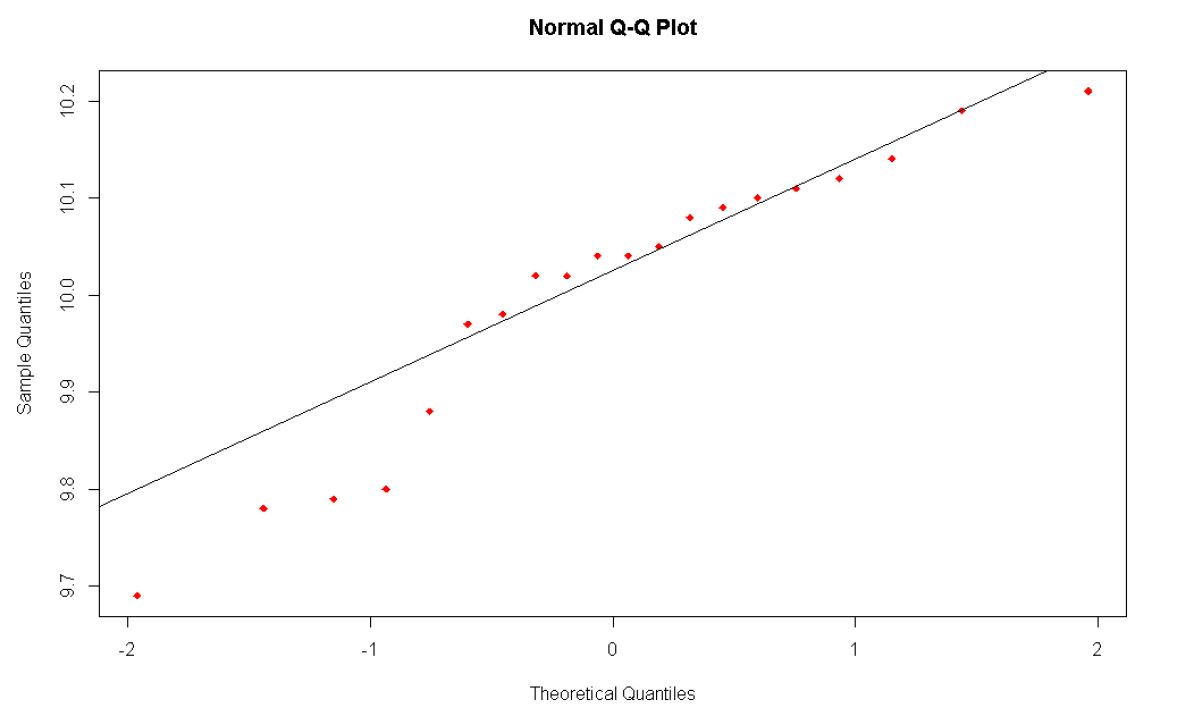
\includegraphics[scale=0.5]{QQplot1}
	\end{center}
\begin{itemize}
	\item Can assume \textbf{Verbal SAT} is a normally distributed variable.
	\item Can not assume \textbf{GPA} is a normally distributed variable.
\end{itemize}
\end{frame}

\end{document}